\section*{Решения и комментарии}

\subsubsection*{Два Биксби} % (THE BIXBY BOYS)

Классическая головоломка.
Конечно же, это были тройняшки.
Третий близнец (Арнольд?) учился в другом классе.

\subsubsection*{Свет на чердаке} % (THE ATTIC LAMP SWITCH)

Эта задача пронеслась по миру, как эпидемия гриппа, где-то лет десять тому назад; я не знаю её источника.

Действительно, невозможно определить, какой выключатель подключён к лампочке на чердаке, если всё, что у вас имеется --- это один бит информации, полученный от вашего похода на чердак.
Однако, вы можете добыть больше сведений, если используете ваши руки!
Включите выключатели 1 и 2, подождите несколько минут, затем выключите второй выключатель и идите на чердак.
Если лампочка не горит, но горячая, значит, второй выключатель это то, что мы ищем.
\heart

Если вы не можете дотянуться до лампочки, но обладаете огромным терпением, вы можете добиться того же результата, включив второй выключатель и подождав пару месяцев, затем включить первый выключатель и посетить чердак.
Если лампочка перегорела, то виноват в этом второй выключатель.

\subsubsection*{Бензиновый кризис} %(GASOLINE CRISIS)

Эта задача была известна довольно давно, вы можете найти её, например, в чудесной книге Ласло Ловаса\footnote{L. Lovasz, \emph{Combinatorial Problems and Exercises}.}.
Трюк заключается в следующем:
представьте, что вы начинаете на автозаправке, скажем, №\,1 с достаточным количеством бензина и затем продолжаете свой путь, опустошая каждую автозаправку на кольцевой дороге.
Когда вы вернётесь к заправке №\,1, 
у вас будет столько же бензина, как и в начале пути.

Во время поездки записывайте, сколько бензина у вас остаётся перед каждой заправочной станцией.
Предположим, что это количество минимально перед автозаправкой №\,$k$.
Значит, если вы начнёте с автозаправки №\,$k$ с пустым баком, вы не рискуете оказаться без бензина на дороге между заправочными станциями.\heart

\subsubsection*{Бикфордовы шнуры} %(USES OF FUSES)

Подожгите одновременно оба конца первого шнура и один конец второго.
Когда первый шнур сгорит (через полминуты), подожгите незажжённый конец второго шнура.
К моменту, когда он догорит полностью, пройдёт 45 секунд.
\heart

Несколько лет назад эта и другие задачи о бикфордовых шнурах распространились по миру, как лесной пожар.
Дик Хесс, эксперт по занимательной математике, 
собрал небольшую книжку таких задач.\footnote{D. Hess, J. Slocum, \emph{Shoelace Clock Puzzles}.}
Сам он впервые услышал приведённую выше задачу от Карла Морриса из Гарвардского университета.

Хесс рассматривает бикфордовые шнуры (он их зовёт шнурками) различной длины, но поджигает их только с концов.
Если же вам позволено поджигать шнур во внутренних точках и вы обладаете определённой ловкостью, то можно добиться гораздо большего.
Например, можно отмерить 10 секунд с помощью одного 60-секундного шнура, если зажечь его с обеих концов и в двух внутренних точках, а затем, каждый раз, когда сегмент сгорает, поджигать в новой внутренней точке.
Таким образом, у вас всё время горят три сегмента с двух концов, и шнур сгорает в шесть раз быстрее.

Будет немного суеты под конец и, конечно же, понадобится бесконечное число спичек, чтобы достичь абсолютной точности.

\subsubsection*{Целые числа и прямоугольники} %(INTEGERS AND RECTANGLES)}

Эта задача была предметом особой 
статьи Стэна Вэгона.%
\footnote{S. Wagon \emph{Fourteen proofs of a Result about Tiling a Rectangle,} Am. Math. Mon. Vol. 94, (1987) 601--617.}

Некоторые из решений, предложенных Вэгоном, забавным образом используют мощную математическую технику.
А одно решение не из их числа, предлагает нам следущее:
наложим на большой прямоугольник сетку, состоящую из квадратов со стороной 1/2, так, чтобы нижний левый угол прямоугольника находился в вершине клетки сетки.
Раскрасив клетки сетки в белый и чёрный цвета в шахматном порядке, 
мы видим, что каждый малый прямоугольник ровно наполовину белый и наполовину чёрный.
Следовательно, то же будет верно и для большого прямоугольника.
Но, допустим, высота большого прямоугольника не целое число, тогда часть 
большого прямоугольника между линиями $x=0$ и $x=1/2$ не содержит одинаковое количество белого и чёрного цвета.
Следовательно, основание должно быть целым числом.\heart

Автор книги несёт ответственность за следующее решение, которое вы не найдёте в статье Вэгона.
Пусть $\varepsilon$ существенно меньше, чем наименьшая из сторон прямоугольников разбиения.
Раскрасим каждый малый прямоугольник с целым основанием светло-серым цветом, кроме тёмных горизонтальных полосок шириной $\varepsilon$ вдоль его верхней и нижней сторон.
Раскрасим оставшиеся прямоугольники тёмно-серым, за исключением светлых вертикальных полосок шириной $\varepsilon$ вдоль левой и правой сторон.

%в решении ссылаются на цвета диаграмы, но при печати она станет ч/б
\begin{figure}[h!]
\centering
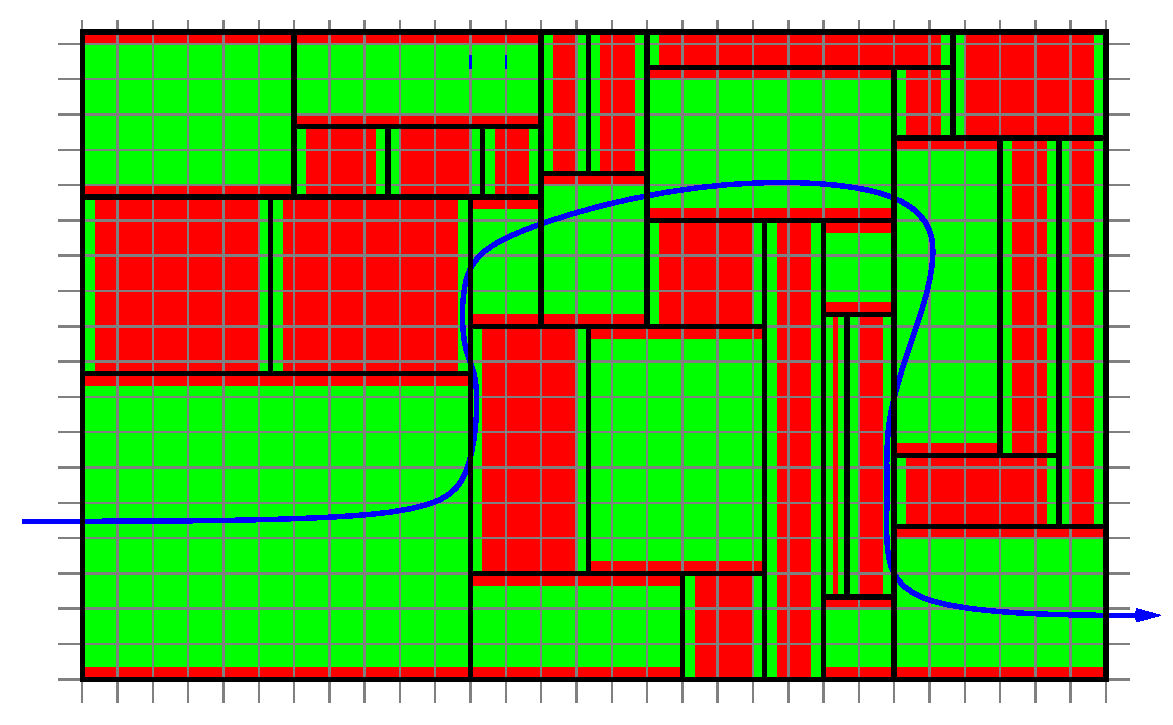
\includegraphics[scale=0.5]{Figs/Insight/green}
\end{figure}

Поместим в нижний левый угол большого прямоугольника начало координат.
Заметим, что у нас есть либо светлый путь с левой стороны большого прямоугольника до его правой стороны, либо тёмный путь с нижней стороны до верхней.
Рассмотрим первый вариант.
Каждое место пересечения светлого пути с вертикальными сторонами малых прямоугольников имеет целую координату; таким образом, основание большого прямоугольника --- целое число.
Подобным же образом и тёмный путь снизу вверх даёт целую высоту.

\subsubsection*{Весы и гири} %(TIPPING THE SCALES)

Рассмотрим результат для каждого подмножества учеников, включая пустое.
Заметьте, что каждая гиря окажется на левой чашке весов ровно в половине случаев.
В частности, средний вес гирь на левой чашке для всех подмножеств учеников равен их среднему весу на правой чашке.
Поскольку для пустого множества правая чашка тяжелее, 
для какого-то другого множества тяжелее должна быть левая.\heart

\noindent{\small Источник: Вторая Всесоюзная математическая олимпиада, Ленинград, 1968.}

Техника «усреднения», описанная выше, часто используется: будьте внимательны!

\subsubsection*{Часы на столе} %(WATCHERS ON THE TABLE)

Рассматривая только одни часы, 
мы видим, что в течении одного часа среднее расстояние от центра стола $C$ до кончика минутной стрелки $M$ превышает расстояние от $C$ до центра часов $W$.
Действительно, если провести через точку $C$ прямую $L$, перпендикулярную прямой $CW$, 
то среднее расстояние от прямой $L$ до точки $M$, очевидно, равно $LW$, 
что, в свою очередь, равно $CW$.
Но расстояние $CM$, по меньшей мере, равно $LM$, а обычно больше.

Взяв сумму по всем часам, приходим к аналогичному заключению, и отсюда следует, что есть момент в течении одного часа, когда желанное неравенство выполняется.\heart

\begin{figure}[h!]
\centering
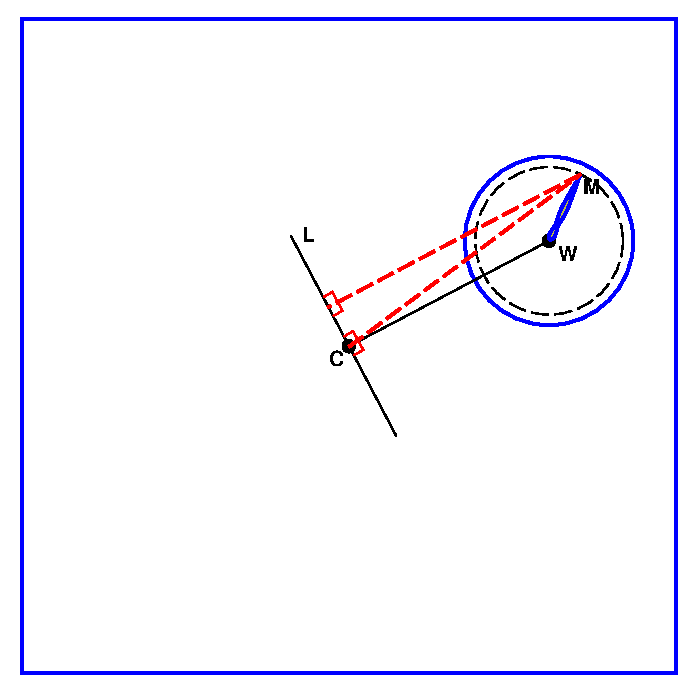
\includegraphics[scale=0.9]{Figs/Insight/watch}
\end{figure}

Требование точности часов обеспечивает движение каждой минутной стрелки с постоянной скоростью.
Это не так уж важно, когда скорости различаются, если только наше терпение не ограничено одним часом.

Одно дополнительное замечание: если установить и расположить часы определённым образом,
то \emph{можно} добиться того, что сумма расстояний от центра стола до кончиков минутных стрелок всегда была строго больше, чем сумма расстояний от центра стола до центров часов.\heart

\noindent{\smallИсточник: данная задача впервые появилась на десятой Всесоюзной математической олимпиаде в Душанбе, 1976.}

\subsubsection*{Путь по шахматной доске} %(PATH ON CHESSBOARD)

Если $n$ --- чётное число, у Боба имеется простая выигрышная стратегия, независимо от того, где Алиса начинает.
Он просто представляет себе, что шахматная доска покрыта прямоугольничками размером $1{\times2}$ клетки (домино) и каждый раз ставит фишку на вторую клетку того домино, куда пошла Алиса («закрывает» домино). %???обычно говорят «доминошки»
(Заметим, что эта стратегия работает для Боба, даже если Алисе разрешено ставить фишку на любую клетку при каждом ходе!).

Если $n$ --- нечётное, и Алиса начинает с угла, она выигрывает, если представит, что домино покрывает всю доску, кроме угловой клетки, с которой она начинает.

Tем не менее, Алиса проигрывает в случае с нечётным $n$, если она должна начинать с клетки, соседней к угловой.
Предположим, угловые клетки на данной доске чёрные, то есть Алиса начинает с белой клетки.
Существует покрытие всей шахматной доски домино, за исключением одной чёрной клетки.
Боб выигрывает, «закрывая» все домино.
Алиса
никогда не сможет поставить фишку на незакрытую клетку, потому что все клетки, на которые она ходит --- белые.\heart

\noindent{\small Источник: Двенадцатая Всесоюзная математическая олимпиада, Ташкент, 1978.}

\subsubsection*{Степень в степени} %(EXPONENT UPON EXPONENT)

Если выражение
$${\sqrt{2}}^{{\sqrt{2}}^{{\sqrt{2}}^{{\cdot}^{\cdot^{\cdot}}}}}$$
имеет какой-то смысл, то это не что иное, как предел последовательности
$${\sqrt{2}}, {\sqrt{2}}^{{\sqrt{2}}}, {\sqrt{2}}^{{\sqrt{2}}^{{\sqrt{2}}}},\dots$$
Этот предел существует, так как последовательность возрастает и ограничена.

Для доказательства первого утверждения, обозначим эту последовательность
$s_1, s_2,\dots$ и докажем по индукции, что $1<s_i\z<s_{i+1}$
для каждого $i\ge 1$.
Это сделать легко, поскольку \[s_{i+2}=
{\sqrt{2}}^{s_{i+1}}
>{\sqrt{2}}^{s_{i}}
=s_{i+1}.\]

Для нахождения верхней грани, заменим самую верхнюю степень в каждом $s_i$ на б\'{о}льшее число $2$, тогда всё выражение превращается в двойку.

Теперь, когда мы знаем, что предел существует, обозначим его $y$.
Он должен удовлетворять уравнению ${\sqrt{2}}^y=y$.
Рассмотрев уравнение $x=y^{1/y}$, 
можно увидеть, применив элементарный матанализ (приношу извинения!), 
что $x$ строго возрастает при возрастании $y$ до максимума при $y=e$
и после чего убывает.
Таким образом, существует не больше двух значений $y$, для данного $x$, 
и при $x=\sqrt{2}$ нам известны оба: $y=2$ и $y=4$.

Поскольку наша последовательность ограничена сверху двойкой, можно исключить $4$ и, таким образом, $y=2$.\heart

Обобщив приведённое выше доказательство, мы видим, что выражение $x^{x^{x^{{\cdot}^{\cdot}}}}$
имеет смысл и равно наименьшему решению уравнения $x=y^{1/y}$ при $x\le e^{1/e}$.
При $x=e^{1/e}$, выражение равно $e$ но как только $x$ превысит $e^{1/e}$, последовательность устремляется к бесконечности.

\subsubsection*{Солдаты в поле}%(SOLDIERS IN THE FIELD)

Данная задача была представлена на шестой Всероссийской математической олимпиаде в Воронеже, 1966.
Её легче всего решать, начав с двух солдат, находящихся друг от друга на кратчайшем расстоянии.
Ясно, что они присматривают друг другом, и если кто-то ещё смотрит на одного из них, тогда у нас имеется солдат, за которым присматривают дважды и, значит, есть солдат, за которым никто не присматривает.
Если же за этими двумя солдатами больше никто не присматривает, то можно их убрать, не влияя на остальных.

Так как число солдат нечётное, то, применяя и далее это рассуждение, мы, в конце концов, придём к одному солдату, который ни за кем не присматривает --- противоречие.\heart

\subsubsection*{Отрезки и расстояния} %(INTERVALS AND DISTANCES)

{\small Источник: Семнадцатая Всесоюзная математическая олимпиада, Кишинёв, 1983.}

Обозначим через $s_1,\dots,s_k$ длины отрезков множества $S$,
пусть их сумма равна $s$.
Рассмотрим интервал $I_{ij}$, содержащий все расстояния, которые можно получить, взяв первую точку на $i$-том и вторую на $j$-том отрезке множества $S$.
Ясно, что длина $I_{ij}$ равна $s_i+s_j$.
Суммируя по всем парам $i\ne j$, 
каждая длина появляется $k-1$ раз,
таким образом, сумма длин интервалов по всем парам различных отрезков, не превосходит $(k-1) s$.
Расстояния между точками, взятыми из $i$-ого отрезка, имеют значения от $0$ до $s_i$.
Значит, общая длина всех интервалов $I_{ij}$ не превосходит $k s$.
Поскольку $k s\ge 1$, получаем $s\ge 1/k$.
\heart

Равенство достигается, если максимум всех $s_i$ равен $s$, 
то есть если все отрезки, кроме одного, имеют нулевую длину.
Этого можно добиться взяв отрезок $[0,\tfrac1k]$ и добавив изолированные точки
$\tfrac2k,\tfrac3k,\dots,1$ или взяв отрезок $[1-\tfrac1k,1]$ с точками
$0,\tfrac1k,\dots,\tfrac{k-2}k$.

\subsubsection*{Собрать 15} %(SUMMING TO 15)

Быстрый способ решить данную задачу --- это представить, что Алиса и Боб пользуются следующим магическим квадратом:
$$
\begin{matrix}
8&1&6\\
3&5&7\\
4&9&2
\end{matrix}
$$
Так как числа в строчке, столбике и диагонали дают в сумме 15, то можно сказать, что они играют в крестики-нолики! 
Всем известно, что наилучшая игра в крестики-нолики приводит к ничьей,
то есть ответ на наш вопрос --- нет, у Алисы нет выигрышной стратегии.
\heart

Эта забавная игра упоминается во втором томе классической книги Элвина Берлекампа, Джона Конвея и Ричарда Гая.%
\footnote{E. Berlekamp, J. Conway, R. Guy, \emph{Winning Ways for Your Mathematical Plays} Academic Press, 1982; 2nd Edition, A K Peters 2001}
В книге задача приписывается некоему «Э. Периколозо Спорджерси»\footnote{E. Pericoloso Sporgersi}, что выглядит очень подозрительно --- такую надпись можно увидеть в итальянских поездах, она предупреждает пассажиров об опасности высовываться из окна.
